
\section{Ciclo de Vida}



\begin{frame}
 \frametitle{Ciclo de Vida}
 \begin{block}{Definição}
  A organização ou os \textbf{gerentes de projetos} podem \textbf{dividir projetos em fases} para
oferecer melhor controle gerencial com ligações adequadas com as operações em
andamento da organização executora. Coletivamente, \textbf{essas fases são conhecidas
como o ciclo de vida do projeto}.
 \end{block}
\end{frame}


\begin{frame}
 \frametitle{Ciclo de Vida}
 \begin{itemize}
  \item O ciclo de vida do projeto define as fases que conectam o início de um projeto ao seu
final.
%\pause
\item Não existe uma única melhor maneira para definir um ciclo de vida ideal do
projeto.
%\pause
\item As descrições do ciclo de vida do projeto podem ser muito genéricas ou muito
detalhadas. Descrições altamente detalhadas dos ciclos de vida podem incluir
formulários, gráficos e listas de verificação para oferecer estrutura e controle.
 \end{itemize}
\end{frame}

\begin{frame}
 \frametitle{Ciclo de vida do projeto}
\begin{figure}
 \centering
 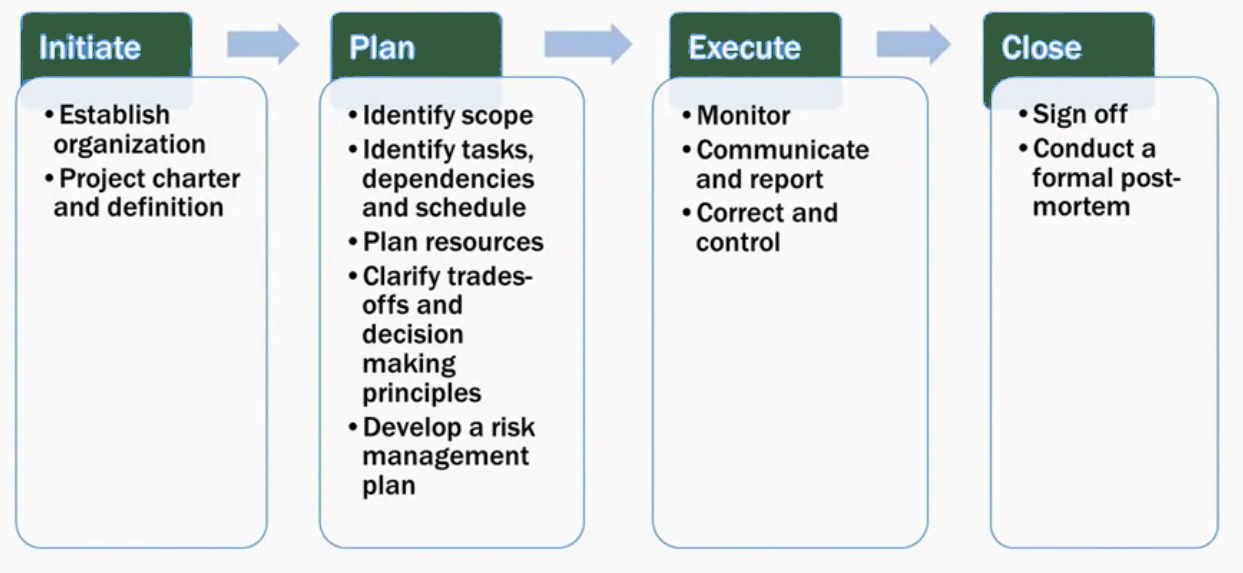
\includegraphics[width = \textwidth]{figs/fig0.png}
\end{figure}
\end{frame}

\begin{frame}
 \frametitle{Ciclo de vida do projeto}
\begin{figure}
 \centering
 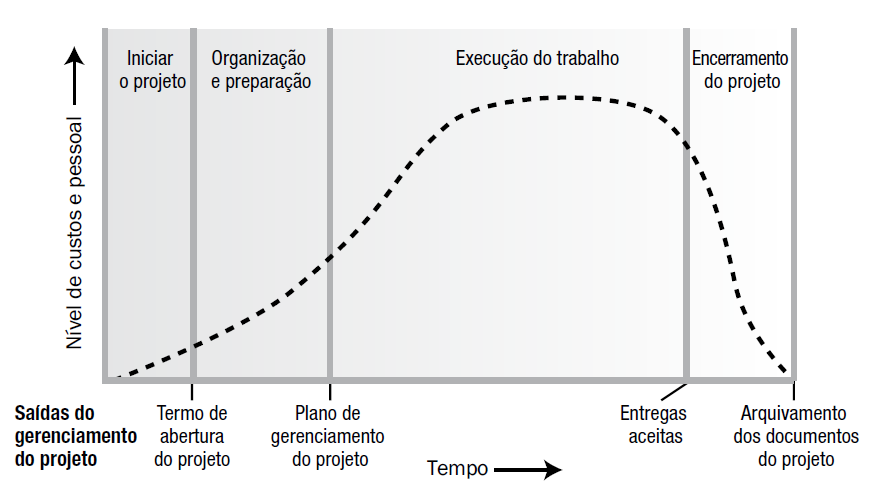
\includegraphics[width = \textwidth]{figs/fig22.png}
\end{figure}
\end{frame}

\begin{frame}
 \frametitle{Os ciclos de vida do projeto geralmente definem}
 \begin{itemize}
  \item Que trabalho técnico deve ser realizado em cada fase
%\pause
\item Quando as entregas devem ser geradas em cada fase e como cada entrega é
revisada, verificada e validada
%\pause
\item Quem está envolvido em cada fase 
%\pause
\item Como controlar e aprovar cada fase
 \end{itemize}
\end{frame}

\begin{frame}
 \frametitle{Ciclo de vida do projeto}
\begin{figure}
 \centering
 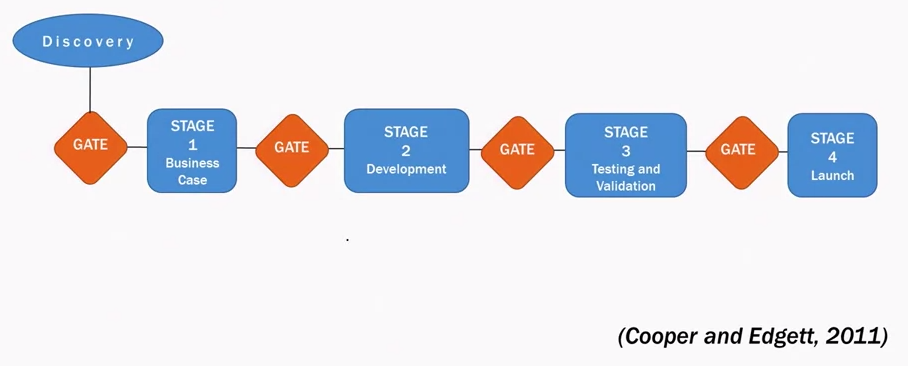
\includegraphics[width = \textwidth]{figs/fig20.png}
\end{figure}
\end{frame}

\section{Projetos e Produto}
\begin{frame}
 \frametitle{Ciclos de vida de projeto e de produto}
 \begin{itemize}
  \item Visão Temporal
  %\pause
  \item Conhecer as fases do ciclo de vida permite:
  \begin{itemize}
   \item Determinar o que foi, ou não, feito pelo projeto;
   %\pause
   \item  Avaliar como o projeto está progredindo até o momento;
   %\pause
   \item  Indicar qual o ponto exato em que o projeto se encontra no momento.
    \end{itemize}
 \end{itemize}
\begin{figure}
 \centering
 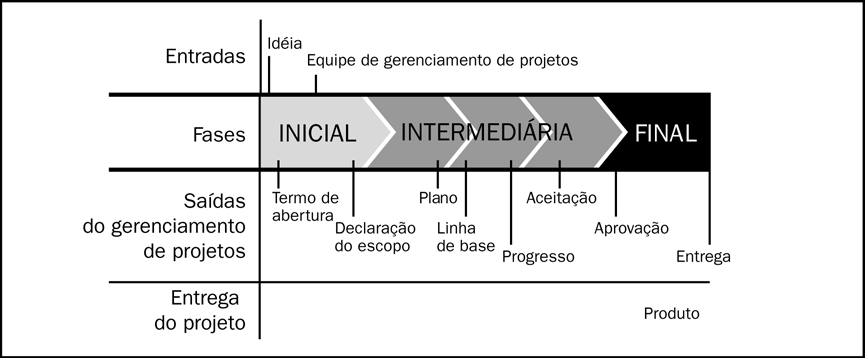
\includegraphics[width = 0.7\textwidth]{figs/ProdCicloVida.png}
 \caption{Relação entre o Produto e os ciclos de vida do projeto}
\end{figure}
\end{frame}

\begin{frame}
 \frametitle{Ciclo de vida do projeto}
 \begin{itemize}
  \item Todo projeto pode ser subdividido em determinadas fases de desenvolvimento
 \end{itemize}
\begin{figure}
 \centering
 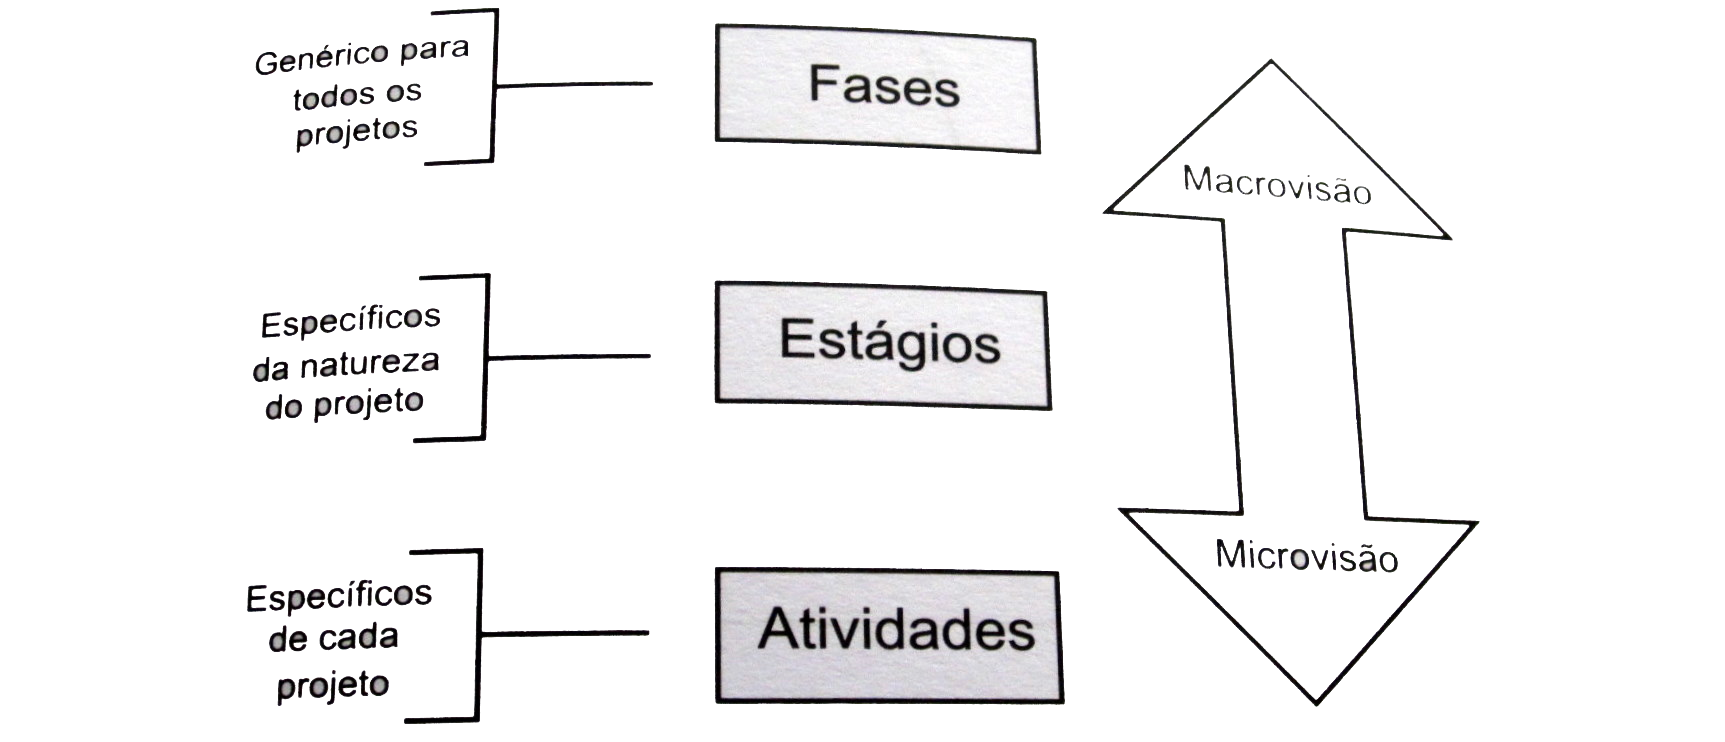
\includegraphics[width = 0.8\textwidth]{figs/fig2.png}
\end{figure}
\end{frame}

\begin{frame}
 \frametitle{Características do Ciclo de vida do projeto}
 \begin{itemize}
  \item Meridith afirma
 \end{itemize}
\begin{figure}
 \centering
 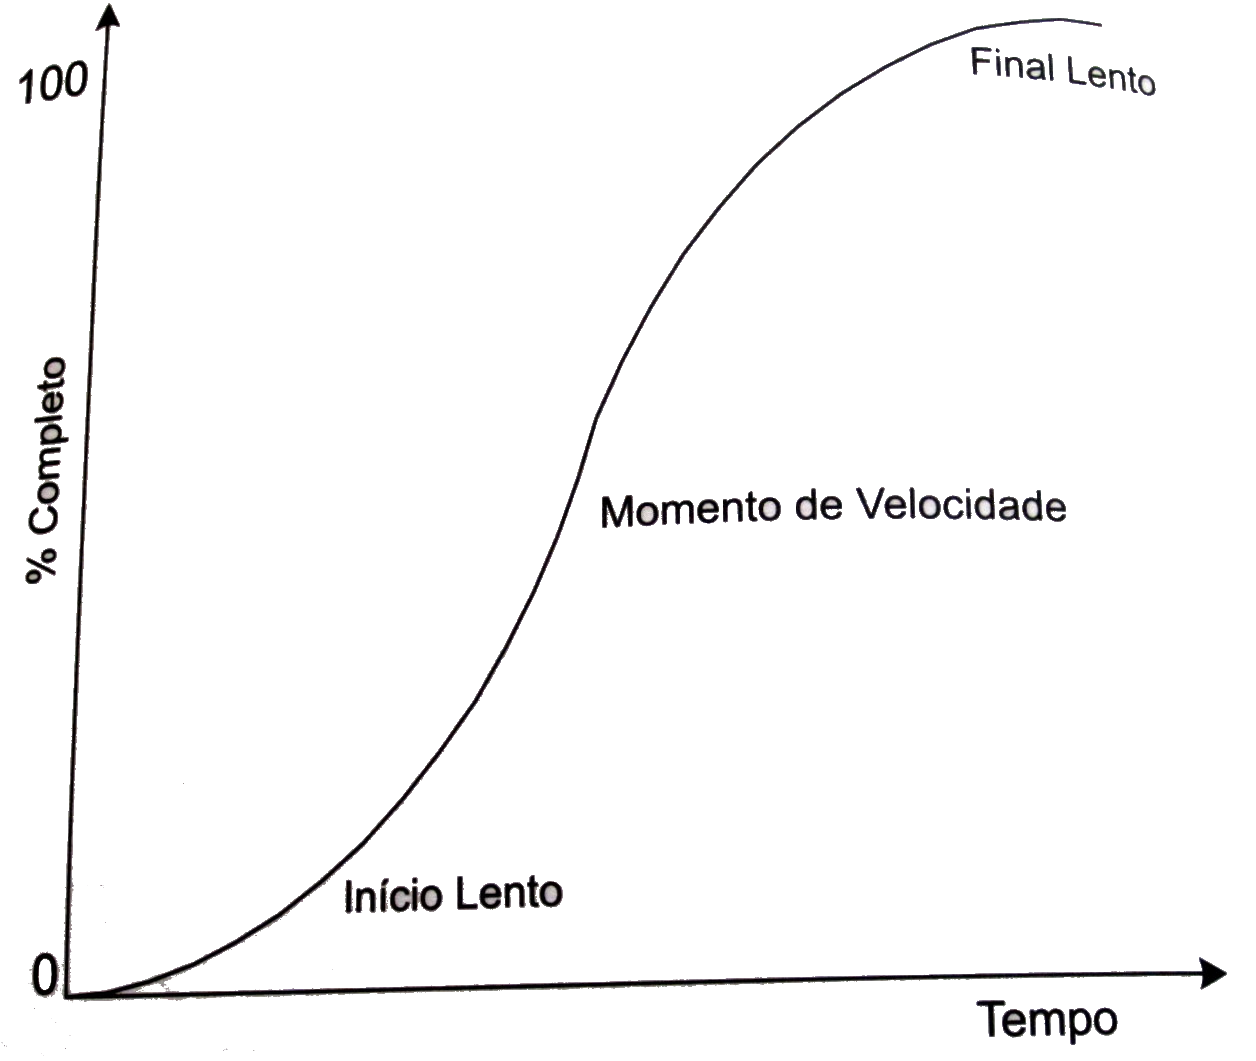
\includegraphics[width = 0.8\textwidth]{figs/fig3.png}
\end{figure}
\end{frame}

\begin{frame}
 \frametitle{Características do Ciclo de vida do projeto}
\begin{itemize}
 \item Esforço é a quantidade de pessoas envolvidas no projeto, 
  o dispêndio de trabalho e dinheiro, as preocupações, as complicações, 
  as horas-extras, etc.
\end{itemize}
 \begin{figure}
 \centering
 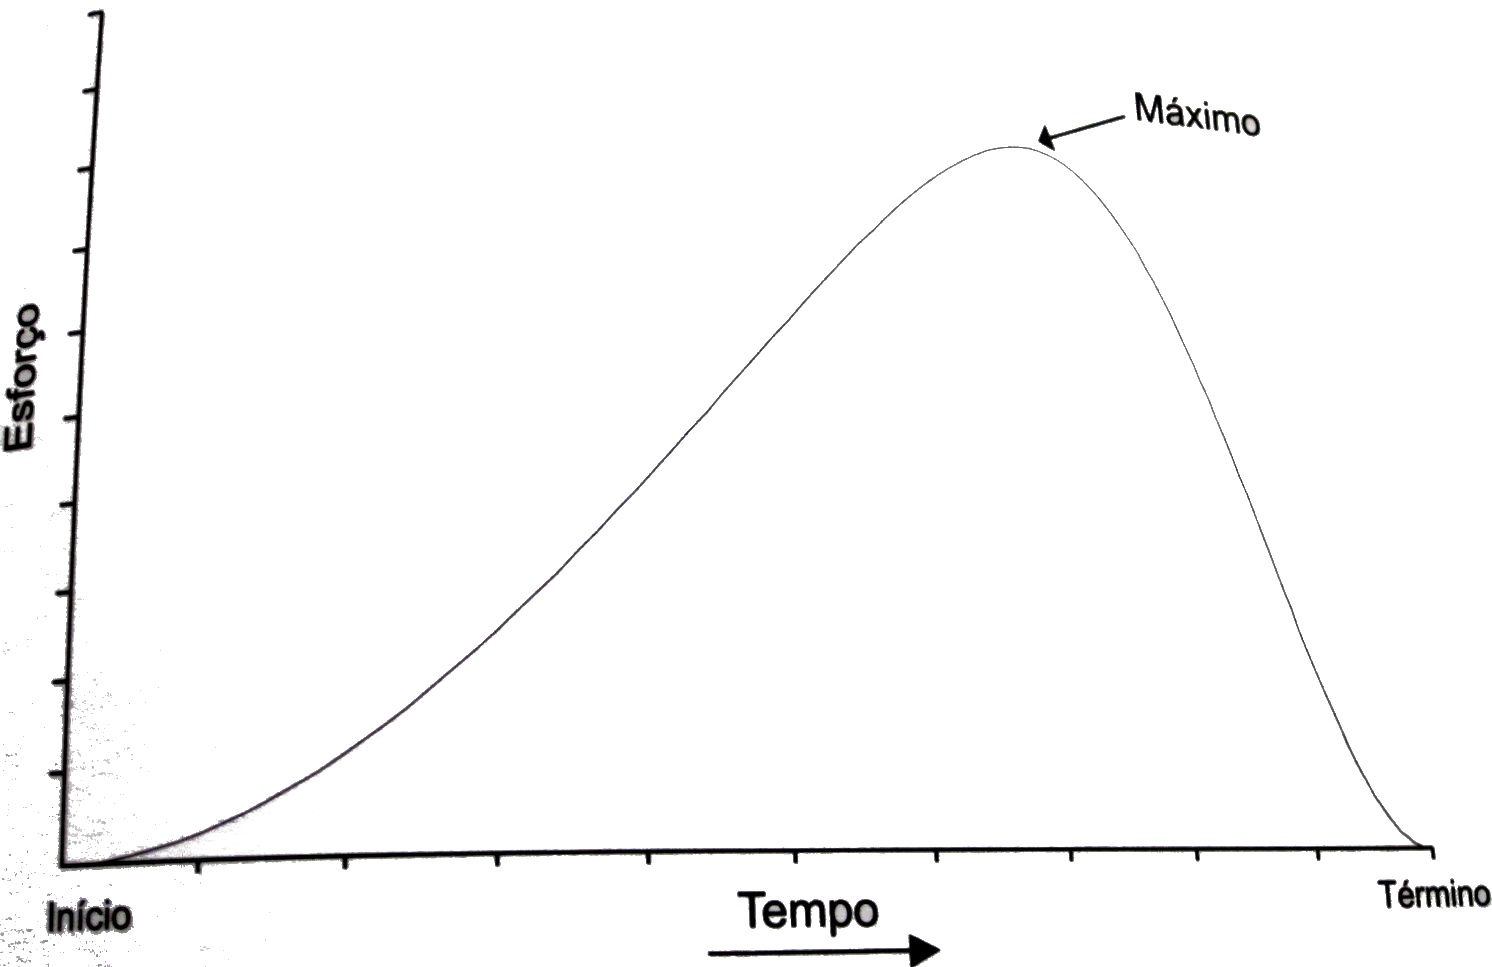
\includegraphics[width = 0.7\textwidth]{figs/fig4.png}
\end{figure}
\end{frame}

\begin{frame}
 \frametitle{Características do Ciclo de vida \\  Potencial de Adicionar Valor}
  \begin{figure}
 \centering
 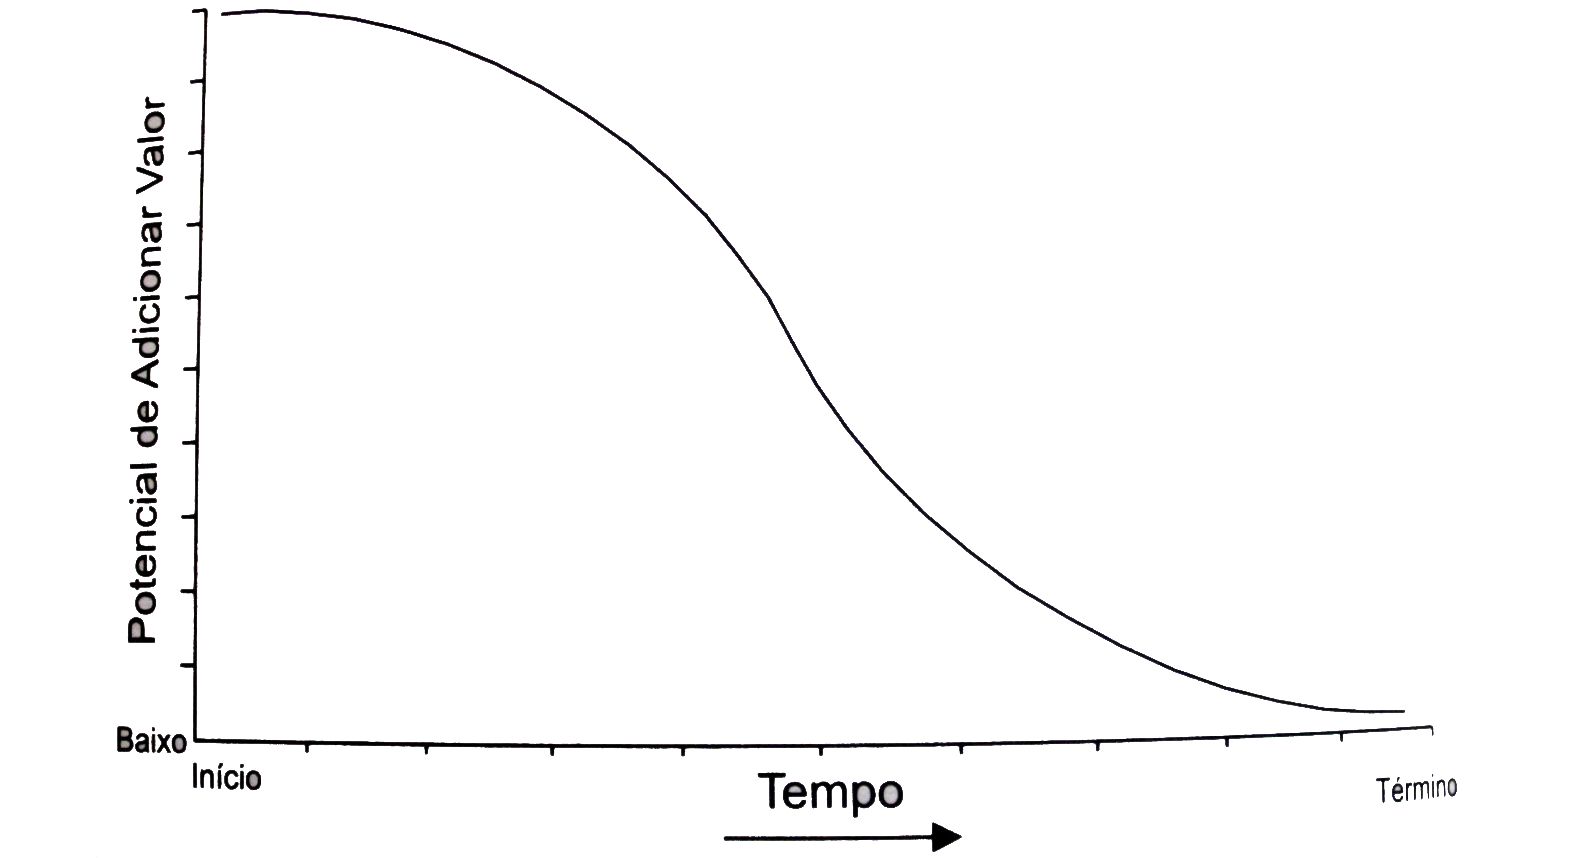
\includegraphics[width = 0.9\textwidth]{figs/fig5.png}
  \end{figure}
\end{frame}

\begin{frame}
 \frametitle{Características do Ciclo de vida  \\ Custo das Mudanças}
  \begin{figure}
 \centering
 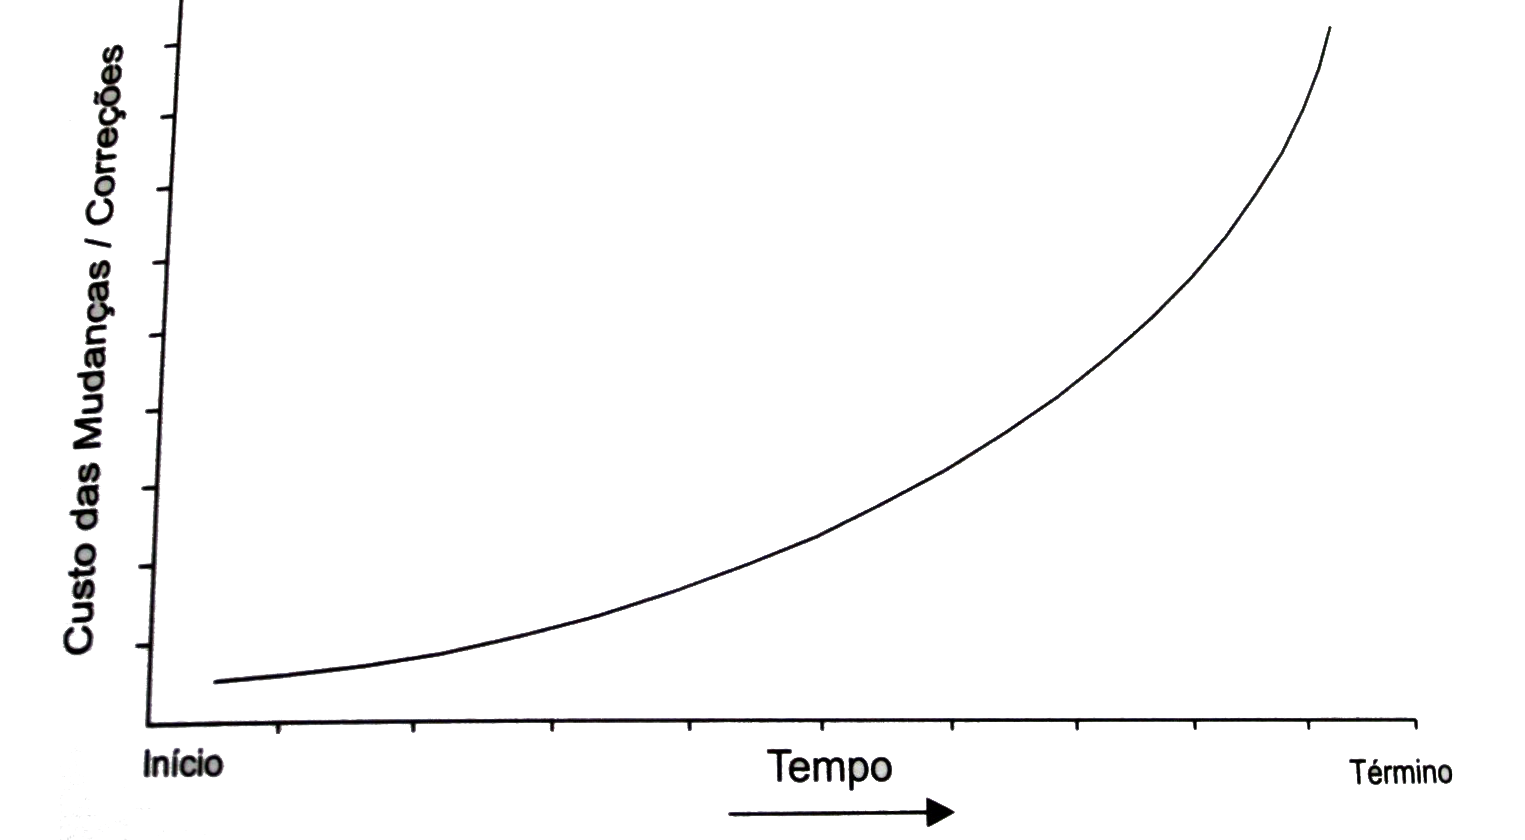
\includegraphics[width = 0.9\textwidth]{figs/fig6.png}
\end{figure}
\end{frame}

\begin{frame}
 \frametitle{Características do Ciclo de vida  \\ \small{Oportunidade Construtiva X Intervenção Destrutiva}}
  \begin{figure}
 \centering
 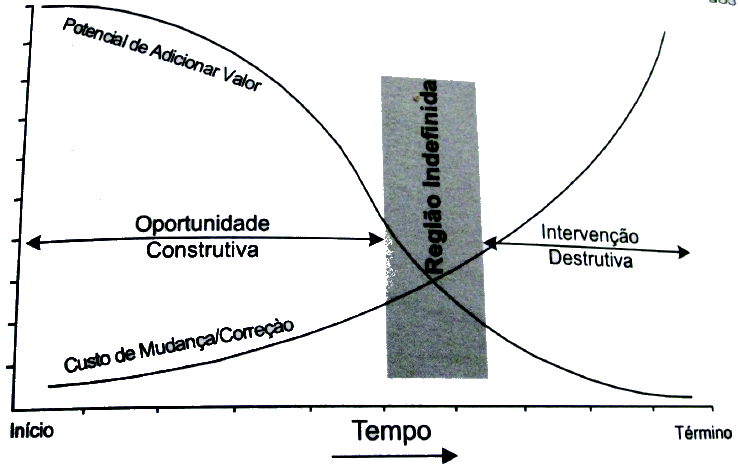
\includegraphics[width = 0.9\textwidth]{figs/fig21.png}
\end{figure}
\end{frame}

\section{Processos de gerenciamento de projeto}
\begin{frame}
 \frametitle{Ciclo de vida \\
 \small{Processos de gerenciamento de projeto}}
 \begin{block}{Processos de gerenciamento de projeto}
  Esses processos garantem o fluxo eficaz do projeto
ao longo da sua existência. Esses processos abrangem as ferramentas e técnicas envolvidas na
aplicação de habilidades e capacidades descritas nas áreas de conhecimento
 \end{block}
\end{frame}

\begin{frame}
 \frametitle{PMBok - Grupos de processos}
 \begin{itemize}
  \item Os grupos de processos  não são fases  do ciclo de vida do projeto
  \begin{itemize}
   \item Projetos grandes  ou complexos podem ser separados em fases ou subprojetos distintos
   \begin{itemize}
    \item Estudos de viabilidade, desenvolvimento de conceitos, projeto, elaboração de protótipo, construção, testes, etc
   \end{itemize}
  \item Todos os processos do grupo de processos são repetidos para cada fase ou subprojeto
  \end{itemize}
  \end{itemize}
\end{frame}

\begin{frame}
 \frametitle{Interações comuns em processos de gerenciamento de projetos}
  \centering
  \begin{figure}
 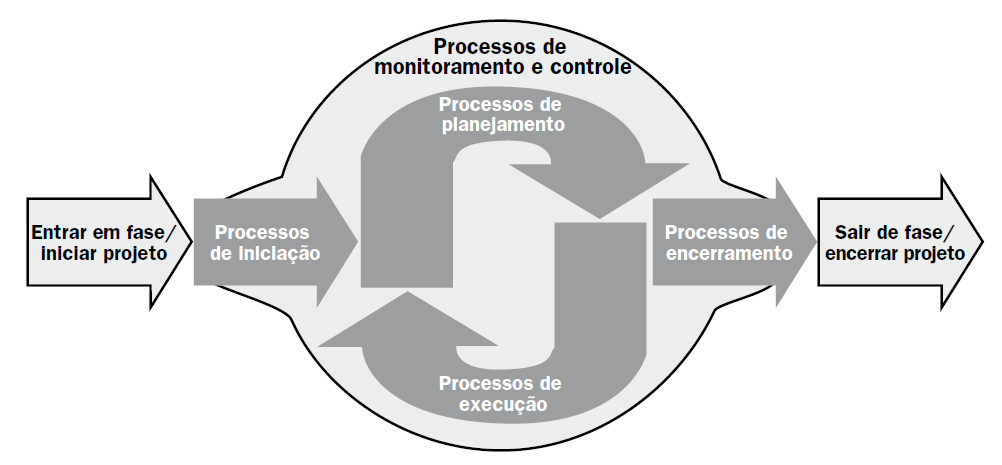
\includegraphics[width = 0.9\textwidth]{figs/fig12_v2.png}
\end{figure}
\end{frame}

\begin{frame}
 \frametitle{Interações comuns em processos de gerenciamento de projetos - PMBOK}
  \centering
  \begin{figure}
 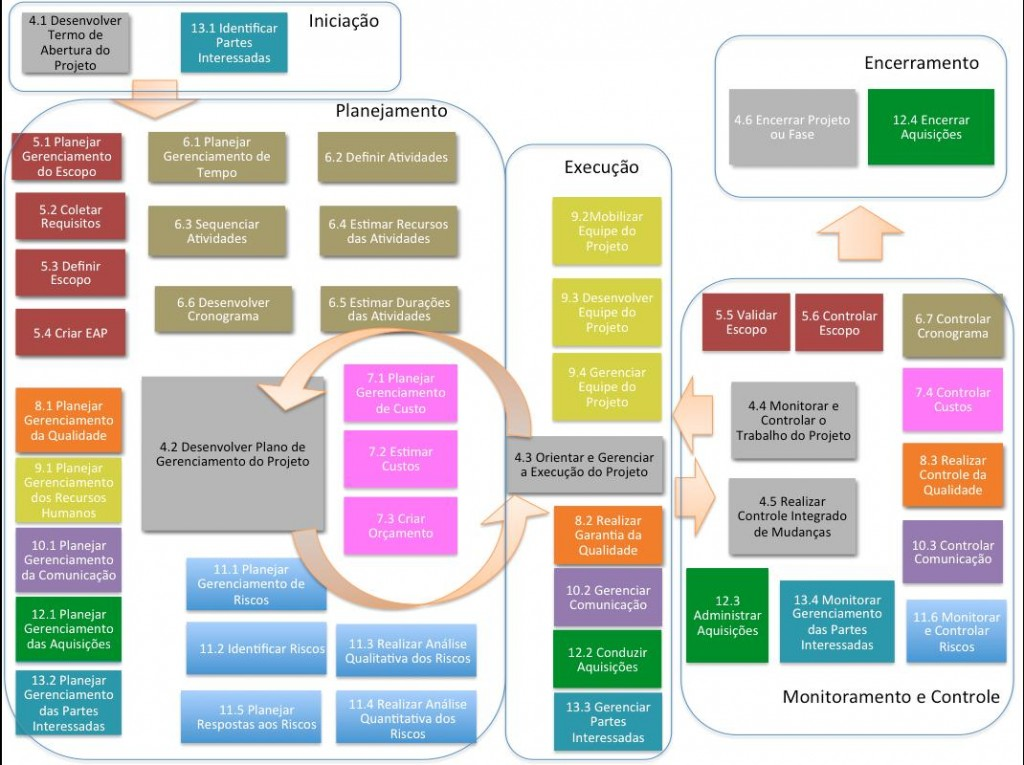
\includegraphics[width = 0.9\textwidth]{figs/figura-4-1024x765.jpg}
\end{figure}
\end{frame}



\begin{frame}
 \frametitle{PMBok - Grupos de processos}
 \begin{itemize}
  \item Grupo de processos de Inicialização
  \begin{itemize}
   \item Define e autoriza o projeto ou uma fase do projeto
  \end{itemize}
  
  \item Grupo de processos de planejamento
  \begin{itemize}
   \item Define e refina os objetivos e planeja a ação necessária para alcançar os objetivos e o escopo para as quais o projeto foi realizado
  \end{itemize}
 
 \item Grupo de processos de execução
  \begin{itemize}
   \item Integra pessoas e outros recursos para realizar o plano de gerenciamento do projeto para o projeto
  \end{itemize}

  \end{itemize}

\end{frame}

\begin{frame}
 \frametitle{PMBok - Grupos de processos}
 \begin{itemize}
  \item Grupo de processos de monitoramento e controle
  \begin{itemize}
   \item Mede e monitora regularmente o progresso para identificar variações em relação ao plano de gerenciamento do projeto, de forma que possam ser tomadas ações
   corretivas quando necessário  para atender os objetivos do projeto
  \end{itemize}
  \item Grupo de processos de encerramento
  \begin{itemize}
   \item Formaliza a aceitação do produto, serviço ou resultado e conduz o projeto ou fase do projeto a um final ordenado
  \end{itemize}
  \end{itemize}

\end{frame}

\begin{frame}
 \frametitle{Processos de Gerenciamento de Projetos - \\
 \small{Grupo de Processos} }
 \begin{figure}
  \centering
  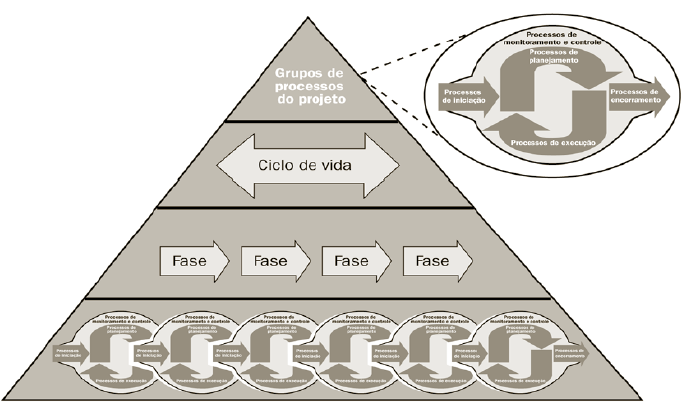
\includegraphics[width = 0.8\textwidth]{figs/fig1_4.png}
 \end{figure}
\end{frame}

\section{Desempenho}
\begin{frame}
 \frametitle{Integração entre Desempenho, Custo e Tempo}
 \begin{block}{Tripla Restrição}
  Necessidades conflitantes de projetos envolvem uma “tripla restrição” – escopo, tempo e custo
 \end{block}
\end{frame}

\begin{frame}
 \frametitle{Integração entre Desempenho, Custo e Tempo}
\begin{itemize}
 \item É impossível predeterminar todos os fatores simultaneamente! (PCT)
 \begin{block}{}
 $Projeto = f(P,C,T)$ \\
 $P = f(C,T)$ \\
 $C = f(P,T)$ \\ 
 $T = f(P,C)$
 \end{block}
 onde
 \begin{itemize}
  \item  $P$ = Desempenho (Performance)
  \item $C$ = Custo
  \item $T$ = Tempo
 \end{itemize}

\end{itemize}
\end{frame}

\begin{frame}
 \frametitle{Integração entre Desempenho, Custo e Tempo}
   \begin{figure}
 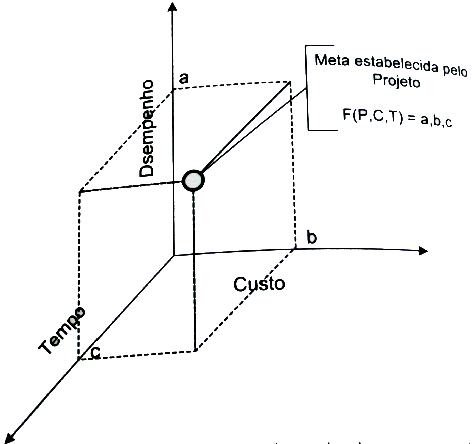
\includegraphics[width = 0.9\textwidth]{figs/fig13.png}
\end{figure}
\end{frame}

\begin{frame}
 \frametitle{Integração entre Desempenho, Custo e Tempo}
 \begin{itemize}
  \item Custo vs Tempo
  \item Desempenho vs Tempo
  \item Desempenho vs Custo
 \end{itemize}

   \begin{figure}
 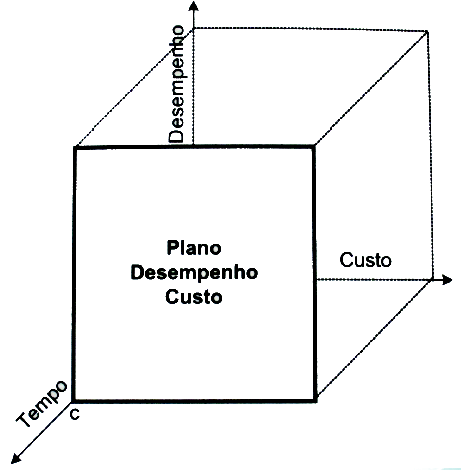
\includegraphics[width = 0.5\textwidth]{figs/fig14.png}
\end{figure}
\end{frame}

\begin{frame}
 \frametitle{Análise de Custo vs Duração Projeto}
   \begin{figure}
 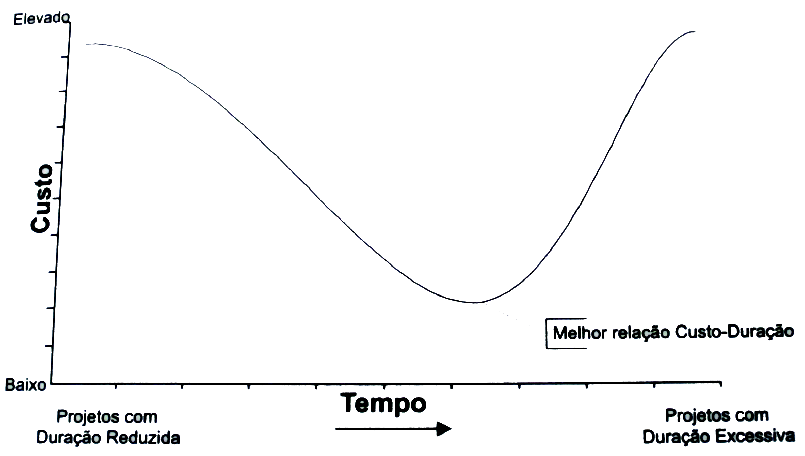
\includegraphics[width = 0.9\textwidth]{figs/fig15.png}
\end{figure}
\end{frame}

\begin{frame}
 \frametitle{Análise de Desempenho vs Duração Projeto}
   \begin{figure}
 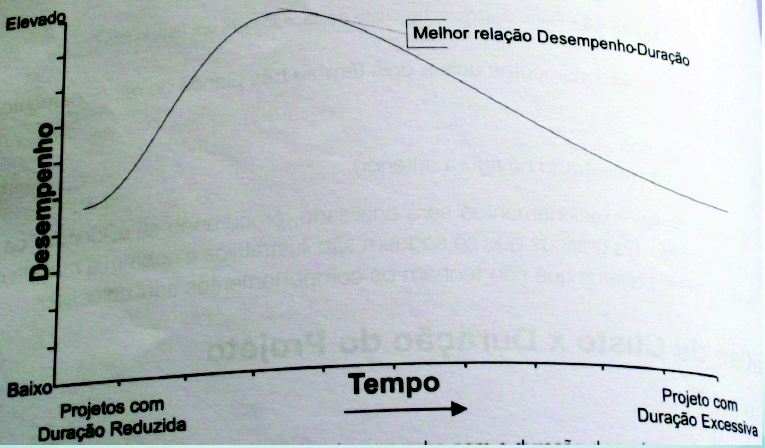
\includegraphics[width = 0.9\textwidth]{figs/fig16.png}
\end{figure}
\end{frame}

\begin{frame}
 \frametitle{Análise de Desempenho vs Investimento}
   \begin{figure}
 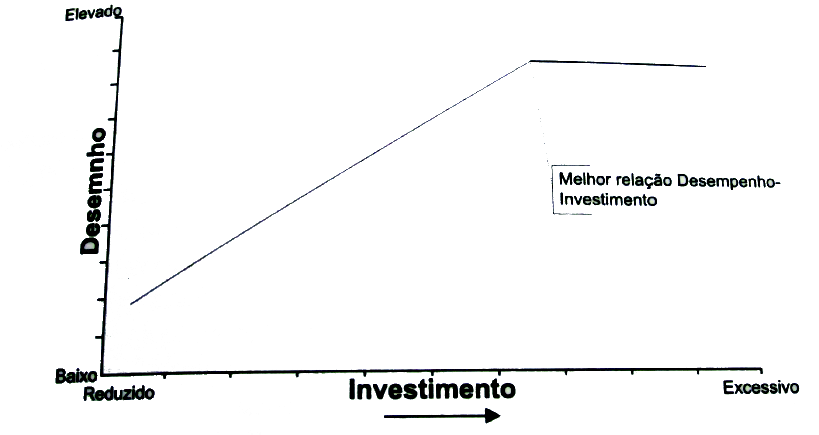
\includegraphics[width = 0.9\textwidth]{figs/fig17.png}
\end{figure}
\end{frame}

\begin{frame}
 \frametitle{Análise de Desempenho vs Escopo}
   \begin{figure}
 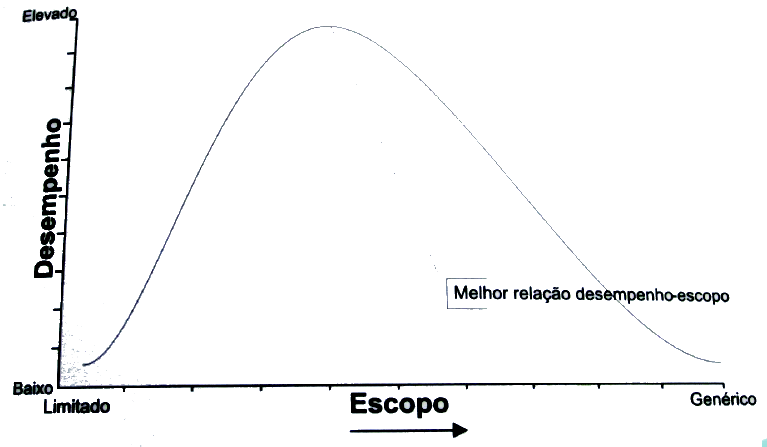
\includegraphics[width = 0.9\textwidth]{figs/fig18.png}
\end{figure}
\end{frame}
\section{Bibliografia}

\begin{frame}
 \frametitle{Bibliografia da Aula \\ 
 Leitura Sugerida}
 \begin{itemize}
  \item \textit{Um guia do Conjunto de Conhecimentos em Gerenciamento de Projetos - guia PMBOK} (Cap. 2)
  \item \textit{https://hbr.org/2014/11/bring-agile-to-the-whole-organization} 
  \item Beware the Next Big Thing - \url{https://hbr.org/2014/05/beware-the-next-big-thing}
 \end{itemize}

\end{frame}

